\documentclass{beamer}

\usepackage{babel}
\usepackage{tikz}
%\usetheme{boxes}
\usepackage[utf8]{inputenc}
\usepackage{amsmath}
\usepackage{amsthm}
\usepackage{hyperref}
\usepackage{natbib}
\usepackage{tikz}
\usepackage{xcolor}
\usepackage[absolute,overlay]{textpos}
\bibliographystyle{plainnat}
\usecolortheme{crane}

\definecolor{orange}{RGB}{232, 86, 15}
\definecolor{blue}{RGB}{14, 159, 232}
\definecolor{blueblue}{RGB}{50, 90, 160}
\definecolor{yellow}{RGB}{232, 187, 14} 
\definecolor{red}{RGB}{232, 14, 59}
\newtheorem{deff}{Definición}
%Information to be included in the title page:
\institute[]{}

\setbeamercolor{title}{bg=blueblue, fg=white}
\setbeamercolor{subttile}{bg=blueblue, fg=white}
\setbeamercolor{frametitle}{bg=blueblue, fg=white}
\setbeamercolor{block title}{bg=blue, fg=white}
\setbeamercolor{block title alerted}{bg=red, fg=white}
\setbeamercolor{block title example}{bg=yellow, fg=white}
\setbeamercolor{footline}{bg=gray, fg=white}
\beamertemplatenavigationsymbolsempty

	
\newcommand{\indep}{\perp \!\!\! \perp}

\newcommand\blfootnote[1]{%
  \begingroup
  \renewcommand\thefootnote{}\footnote{#1}%
  \addtocounter{footnote}{-1}%
  \endgroup
}


\newcommand\overalert[2]{
	 \only<#1>{
\begin{textblock*}{\textwidth}(.35\textwidth,0.25\textheight)
    \begin{beamercolorbox}[wd=.5\textwidth,center,sep=0.3cm]{block title alerted}
	    #2
    \end{beamercolorbox}
\end{textblock*}
}
}

\newcommand\overexample[2]{
	 \only<#1>{
\begin{textblock*}{\textwidth}(.35\textwidth,0.25\textheight)
    \begin{beamercolorbox}[wd=.5\textwidth,center,sep=0.3cm]{block title example}
	    #2
    \end{beamercolorbox}
\end{textblock*}
}
}


\newcommand\overeblock[2]{
	 \only<#1>{
\begin{textblock*}{\textwidth}(.35\textwidth,0.25\textheight)
    \begin{beamercolorbox}[wd=.5\textwidth,center,sep=0.3cm]{block title}
	    #2
    \end{beamercolorbox}
\end{textblock*}
}
}

\title{Causal discovery}
\author{Gherardo Varando}
\date{IPL \\ 09 May 2023}
\begin{document}

\begin{frame}
	\titlepage
\end{frame}


\begin{frame}{Causal Discovery} 
	\begin{columns}
		\begin{column}{0.5\textwidth}
			\begin{itemize}
				\item<1-> Which are the regions most affected by ENSO? 
				\item<2-> Which are the causal drivers and the causal 
					relationships involving food insecurity? 
				\item<3-> Retrieve the reaction network between genes and proteins from single-cell data 
			\end{itemize}
		\end{column}
		\begin{column}{0.5\textwidth}
			\only<1>{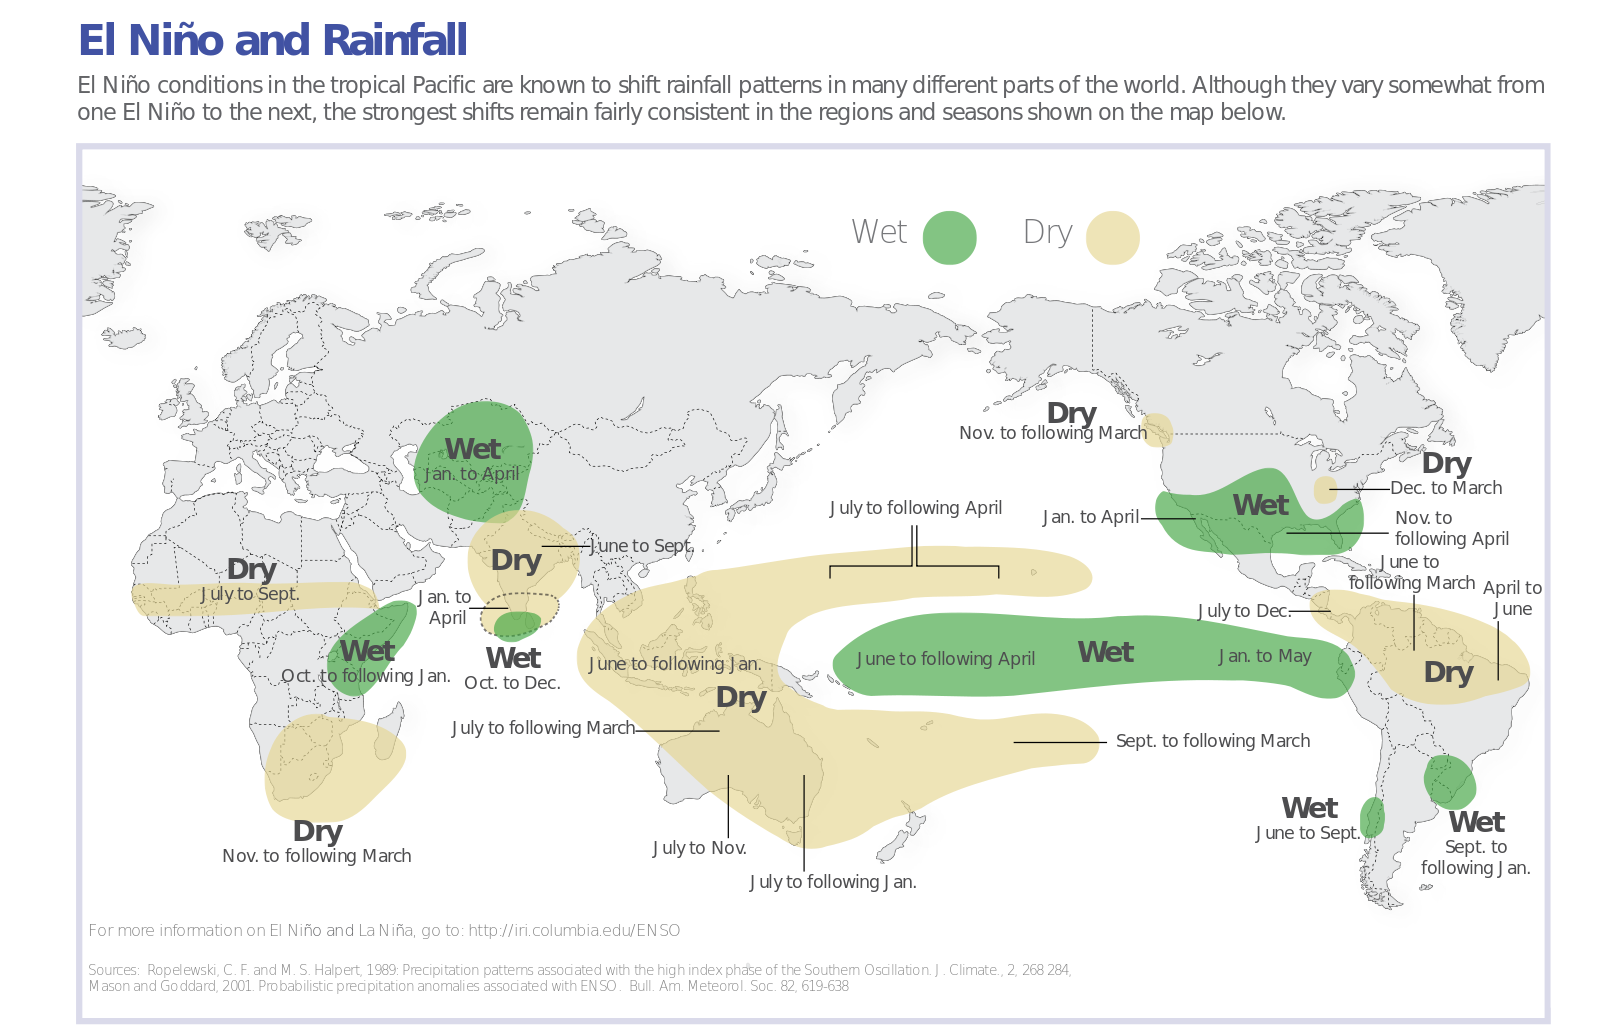
\includegraphics[scale=0.1]{images/enso}}
			\only<2>{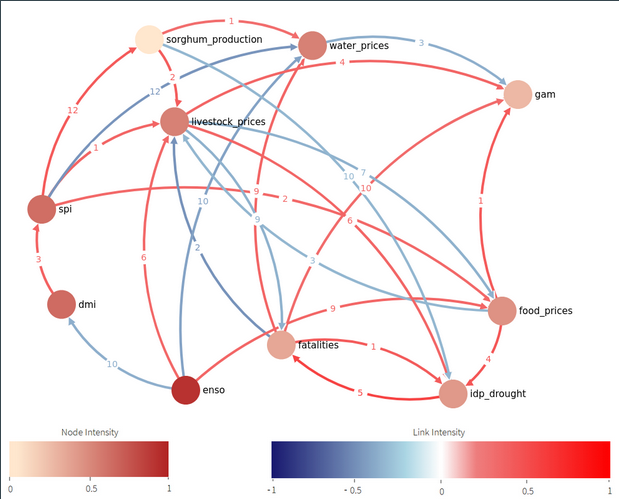
\includegraphics[scale=0.2]{images/baidoa}}
			\only<3>{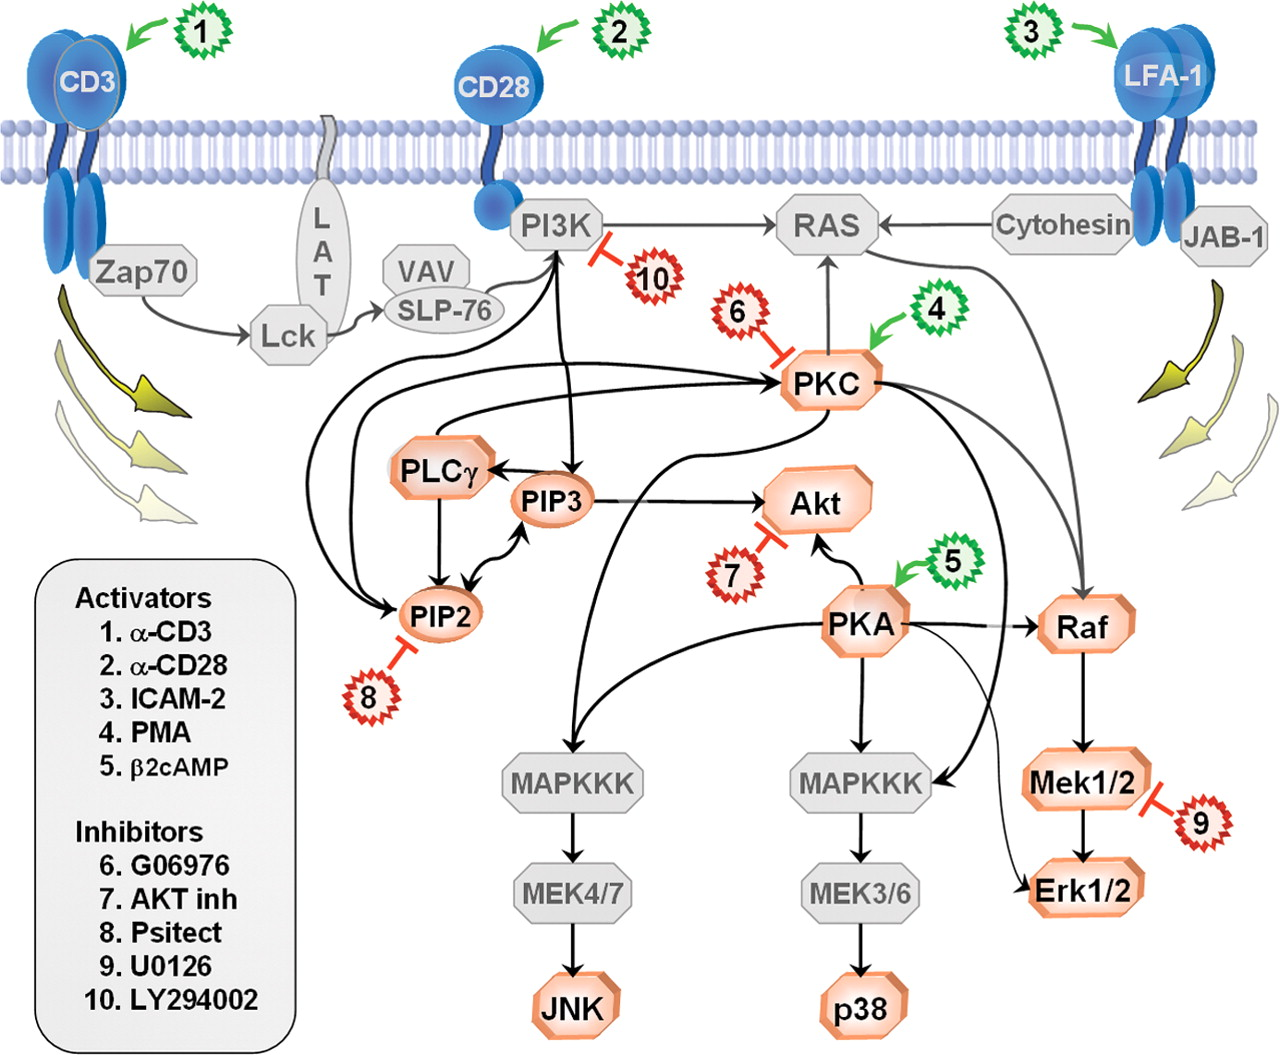
\includegraphics[scale=0.1]{images/grn}}
		\end{column}
	\end{columns}
\end{frame}

\begin{frame}{Causal Discovery} 
	\begin{itemize}
		\item<1-> Learn the structure/graph of the causal relationships between variables 
		\item<2-> If only two variables are considered: bivariate causal discovery 
		\item<3-> it always require assumptions 
		\item<4-> can use only observational data, or even interventions 
		\item<5-> usually the output is not a complete description of the causal relationships 
			  (depends on the assumptions, the type of data etc..) 
	\end{itemize}
\end{frame}


\begin{frame}{Causal discovery methods}
	\begin{itemize}
		\item Constrained Based, Score based, Asymmetry based 
		\item Methods for i.i.d. data or for time-series 
		\item Bivariate vs multivariate
		\item Observational and/or Interventional data  
	\end{itemize}
\end{frame}


\begin{frame}{In this session}
	\begin{itemize}
		\item Causal discovery for BN and SCM
		\item Causal discovery taxonomy 
		\item Some methods 
		\item Examples
	\end{itemize}

	\begin{block}{}
We will see only methods that employ observational data \ldots thus we will need assumptions   
		\end{block}
\end{frame}


\begin{frame}{Structural learning for BN} 
	\begin{block}{}
		Estimate the structure of a BN from observational data. That is,
		recovering of $G$ from 
		(i.i.d.) observations sampled from a probability $P$ such that $(G, P)$ is a BN
	\end{block}
	\begin{itemize}
		\item it is a model selection problem
		\item no causality involved (yet) 
		\item Problem: a probability $P$ can be \emph{comaptible} with multiple BN!! 
	\end{itemize}
\end{frame}

\begin{frame}{Markov equivalence class}
	\begin{itemize}
		\item<1-> $\mathcal{M}(G) = \{P \text{ s.t. satisfies global (or local) Markov  w.r.t. } G\}$ 
		\item<2-> If $\mathcal{M}(G_1) = \mathcal{M}(G_2)$ then we say that $G_1$ and $G_2$ are Markov equivalent. This means $G_1$ and $G_2$ represent the same set of d-separations and thus entails the same set of conditional independence statements 
		\item<3-> A \textbf{Markov equivalence class} contains all graph which are Markov equivalent  
	\end{itemize}
	\onslide<4->\begin{theorem}[\citet{verma1990equivalence}]
Two DAGs $G_1$ and $G_2$
are Markov equivalent if and only if they have the same skeleton and the same
immoralities
	\end{theorem}
	\overexample{5}{Using observational data alone, Can we hope to learn something more than the Markov equivalence class?}  
\end{frame}
\begin{frame}
\begin{theorem}[\citet{verma1990equivalence}]
Two DAGs $G_1$ and $G_2$
are Markov equivalent if and only if they have the same skeleton and the same
immoralities
	\end{theorem}

	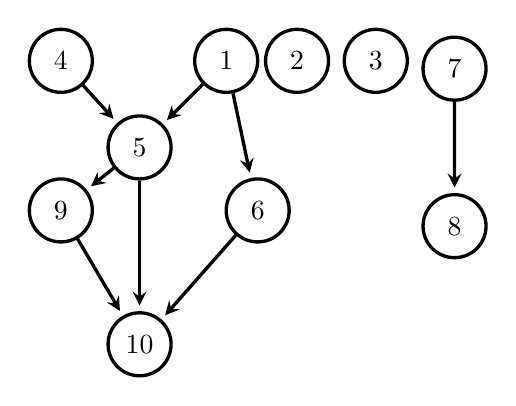
\begin{tikzpicture}[scale=5, 
       node/.style={circle,inner sep=1mm,minimum size=0.8cm,draw,
      very thick,black,fill=white,text=black},
        nondirectional/.style={very thick,black},
        unidirectional/.style={nondirectional,shorten >=2pt,-stealth},
        bidirectional/.style={unidirectional,bend right=10}]

	\node [node] (v1) at (0.420000, 0.720000)       {1};
        \node [node] (v2) at (0.60000, 0.720000)        {2};
        \node [node] (v3) at (0.80000, 0.720000)        {3};
        \node [node] (v4) at (0.00000, 0.720000)        {4};
        \node [node] (v5) at (0.200000, 0.500000)       {5};
        \node [node] (v6) at (0.500000, 0.340000)       {6};
        \node [node] (v7) at (1.000000, 0.700000)       {7};
        \node [node] (v8) at (1.000000, 0.300000)       {8};
        \node [node] (v9) at (0.00000, 0.340000)        {9};
	\node [node] (v10) at (0.200000, 0.000000)      {10};

        \path [unidirectional] (v1) edge (v5);
        \path [unidirectional] (v4) edge (v5);
        \path [unidirectional] (v5) edge (v9);
        \path [unidirectional] (v5) edge (v10);
        \path [unidirectional] (v1) edge (v6);
        \path [unidirectional] (v6) edge (v10);
        \path [unidirectional] (v7) edge (v8);
        \path [unidirectional] (v9) edge (v10);
\end{tikzpicture}

	we can represent the Markov equivalence class with a partial directed acyclic graph (PDAG) 
\end{frame}


\begin{frame}{Taxonomy of methods for BN}
	\begin{itemize}
		\item<1-> Constrained based: PC algorithm 
		\item<2-> Score based or score+search: GES, tabu search, hill-climbing
		\item<3-> hybrid: max-min-hill-climbing (mmhc) 
	\end{itemize}
\end{frame}

\begin{frame}{Constrained based}
	\begin{itemize}
		\item<1-> Start from the full dependency graph 
		\item<2-> prune edges by iteratively test (conditional) independences 
		\item<3-> use some rules to orient edges 
		\item<4-> obtain a PDAG (partial directed acyclic graph) representing the Markov 
			equivalence class
	\end{itemize}
	\blfootnote{\citet{glymour2019review, spirtes2000causation}}
\end{frame}

\begin{frame}
	The PC algorithm starts from a fully connected undirected graph and consists of three phases:
\begin{enumerate}
\item The \emph{skeleton phase} uses statistical (conditional) independence tests to infer the adjacencies of the underlying causal graph. %(which are the same as the adjacencies of the CPDAG).
If two variables $X$ and $Y$ are found to be independent conditional on a (possibly empty) set of variables $\mathbf{Z}$, then the edge between $X$ and $Y$ is removed.
\item The \emph{collider orientation phase} then orients all \emph{collider motifs}, that is, motifs of the form $X \rightarrow Y \leftarrow Z$ where $X$ and $Z$ are non-adjacent. These orientations can be inferred because collider motifs impose a particular pattern of (conditional) (in-)dependencies.
\item The \emph{orientation phase} finally uses graphical rules \citep{meek1995causal} to infer the orientation of as many remaining unoriented edges as possible using the acyclicity assumption and the fact that all colliders have been found in the previous step.
\end{enumerate}
\end{frame}


\begin{frame}{Score based}
	\begin{itemize}
		\item<1-> find the \textbf{best scoring graph} with respect to some scoring criteria (e.g. BIC) 
		\item<2-> space of DAGs is huge .... we need heuristic searches  
		\item<3-> hill-climbing, tabu search 

		\item<4-> GES (greedy equivalent search) in the space of CPDAG (the space of Markov equivalence classes) [under some assumpotions it is proven to recover the true Markov equivalence class] 
	\end{itemize}
	\blfootnote{\citet{chickering2002optimal}}
\end{frame}

\begin{frame}{Causal discovery methods}
	\begin{itemize}
		\item Constrained Based, Score based, Asymmetry based 
		\item Methods for i.i.d. data or for time-series 
		\item Bivariate vs multivariate
		\item Observational and/or Interventional data  
	\end{itemize}
\end{frame}


\begin{frame}{Asymmetry based methods} 
	\begin{itemize}
		\item<1-> Use assumptions on the SCM to infer causal structure 
		\item<2-> Can distinguish graphs in the same Markov equivalence class 
		\item<3-> Developed especially in the bivariate setting (but also in multivariate case)
		\item<4-> example, Linear non-Gaussian acyclic model (LiNGAM)~\citep{shimizu2006linear} 
	\end{itemize}
\end{frame}


\begin{frame}{Time series}
\begin{itemize}
	\item Causal discovery in time series can be \emph{easier} then i.i.d. case 
	\item The \emph{arrow of time} helps in orienting some edges 
	\item<2-> Granger causality, convergent cross-mapping (CCM), PC-based methods (PCMCI), 
		score-based methods, (VAR)LinGAM, TiMINO, \ldots 
\end{itemize}
\end{frame}


\begin{frame}{Granger causality} 
\begin{block}{Granger causality}
$A(t)$ is linearly Granger-cause of $B(t)$ with 
respect to a fixed time-lag $m$ 
if the null hypothesis 
$\left\{ \alpha_\ell=0 \,\text{for}\, \ell = 1,\ldots,m \right\}$ 
is rejected for the linear AR model 
		\[B(t) = \sum_{\ell=1}^m \beta_\ell B(t-\ell) + \sum_{\ell=1}^m \alpha_\ell A(t-\ell) + \beta_0 + \epsilon.\]
	\end{block}
\end{frame}


\begin{frame}[allowframebreaks]
\bibliography{biblio}
\end{frame}

\end{document}


